\chapter{Preliminaries}
\label{chap:intro}
This thesis is principally focussed on extracting quantitative information
from \ac{NMR} data. In this first chapter, concepts are introduced to help
contextualise the work undertaken.
After a brief introduction to \ac{NMR}, including key historical developments
and a simple description of its theoretical underpinnings, focus turns to
the form that \ac{NMR} data takes. The means by which said data is
conventionally processed and analysed to gain chemical insights is discussed.
Techniques which estimate the parameters which describe \ac{NMR} data based on
a model of summed complex sinusoids are an alternate means of analysing
\ac{NMR} data. While able to afford richer information than conventional
approaches, these are not widely employed in \ac{NMR}, despite many effective
methods existing. A review of some of the most prominent ones are given.
Finally, the motivation for the project undertaken is discussed, and an outline of
the rest of the thesis is given.

\section{An Introduction to \acs{NMR}}

\subsection{A Brief History}
Since its conception almost 80 years ago, \ac{NMR} has become a ubiquitous
technique in chemistry, biochemistry and numerous other disciplines, thanks to
the unique insights into chemical structure and dynamics that it
can provide.
The origins of the subject can be traced back to 1945, when independent work by
Felix Bloch on water~\cite{Bloch1946} and Edward Purcell on
paraffin~\cite{Purcell1946} gave rise to the first illustrations of nuclear
magnetic resonances in condensed phases. The two hadn't met before their
respective papers were published with about a month's
separation~\cite{Becker1993}. Both received the Nobel Prize in Physics in 1952
``for their development of new methods for nuclear magnetic precision
measurements and discoveries in connection therewith''~\cite{Nobel1952}. A
notable mention should also be given
to Yevgeny Zavoisky, the father of the related field of electron paramagnetic
resonance, who probably observed NMR as far back as 1941,
though he dismissed his results as irreproducible~\cite{Eaton1998}. A few years
subsequently, works investigating
\ac{NMR} spectra from compounds containing nuclei such as \ch{^{63}Cu},
\ch{^{65}Cu}, \ch{^{31}P}, \ch{^{14}N}, and \ch{^{19}F} led to an
understanding of the \emph{chemical shift}, a phenomenon in
which nuclei in different chemical environments exhibit
non-identical resonant frequencies~\cite{Knight1949, Proctor1950,
Dickinson1950}.  Chemists regarded these findings with great
interest, as they suggested that \ac{NMR} could give insights into molecular
structure.

Russell Varian\,---\,founder of \textsc{Varian Associates} along with his brother
Sigurd\,---\,
secured the first patent for a commercial \ac{NMR} machine, with
a \qty{30}{\mega\hertz} spectrometer following soon after. The first
spectrometers functioned by gradually varying the magnetic field strength,
causing spins to come into resonance at different times, in a process referred
to as continuous wave spectroscopy. Richard Ernst and
Weston Anderson, working at \textsc{Varian} at the time, proposed an alternative
method: pulsed \ac{FT} spectroscopy~\cite{Ernst1966}. This was not seen as a
fruitful endeavour by the company, largely because of the very long time it
took to digitise the signal, and subsequently compute its FT~\cite{Freeman2015}.
Instead, the first commercial pulsed \ac{FT} spectrometer was produced by
\textsc{Bruker Corp.} in 1969, which revolutionised NMR. The innovation emerged
shortly after Cooley and Tukey's introduction of the \ac{FFT}
algorithm~\cite{Cooley1965}, which incentivised the use of the pulsed
\ac{FT} approach.

The concept of \ac{2D} \ac{NMR} spectroscopy was proposed by Jean Jeener in
1971~\cite{Jeener1971, Jeener2016}, which Ernst and co-workers showcased a few
years later in the form of a \ac{COSY} experiment~\cite{Aue1976a}. The use of
multiple dimensions to spread out signals enabled vastly more complex
structures to be studied. In 1985, the first protein assignment by
\ac{NMR}\,---\,using \ac{COSY} and \ac{NOESY} experiments\,---\,was reported
by Kurt W\"uthrich and co-workers~\cite{Williamson1985}. Over time, there have
been extensive developments in techniques for biomolecular systems, including
the creation of 3D and 4D ``triple resonance'' experiments~\cite{Marion1989,
Kay1990}, as well \ac{TROSY} experiments~\cite{Pervushin1997} for the study of
large proteins.

\ac{NMR}'s significance as an analytical tool is evidenced by Nobel Prizes in
Chemistry being awarded for work in the field on two separate occasions, on top
of the 1952 Physics Prize. First,
Ernst received the prize in 1991 ``for his contributions to the development of
the methodology of high resolution \acl{NMR}"~\cite{Ernst1992}. In 2002,
W\"uthrich was recognised ``for his development of \acl{NMR} for determining
the three-dimensional structure of biological macromolecules in
solution"~\cite{Wuthrich2003}.

\subsection{The Bloch Model}

\ac{NMR} relies on an intrinsic property of \correction{nuclei with an odd number of
protons and/or neutrons}\label{corr:prot-neut} called \textit{spin}
which, along with orbital angular momentum \correction{and molecular rotation, is one of
the sources}\label{corr:mol-rot} of angular momentum in quantum mechanics.
The angular momentum associated with a nuclear spin is characterised by the
quantum number $I \in \lbrace 0, \nicefrac{1}{2}, 1, \nicefrac{3}{2}, \cdots
\rbrace$. Spin-\nicefrac{1}{2}
nuclei are the most commonly studied in \ac{NMR}, as those with $I >
\nicefrac{1}{2}$ often have very short-lived excited states due to electric
quadrupole effects. A rigorous description of \ac{NMR} requires the application
of quantum mechanics, with many excellent texts on the subject available to
suit newcomers and experts alike; notable examples include the
following citations (in approximate order of complexity):
~\cite{Hore2015,Levitt2007,Cavanagh2007,Goldman1988,Abragam1961,Kuprov2023}.
Despite this, a basic
appreciation can be gained using the Bloch (vector) model, a semi-classical
description of the simplest possible system to study: a ensemble of
isolated, identical spin-$\nicefrac{1}{2}$ nuclei~\cite[Chapter 1]{Hore2015}.
The Bloch model becomes inadequate when more complex spin systems are
considered, featuring non-identical spins which interact through mechanisms
such as scalar couplings (commonly referred to as J-couplings), dipolar
couplings etc. However, it provides valuable insights into the basic principles
of \ac{NMR}, including the form that a typical dataset acquired by an
experiment takes.

The nuclear spin angular momentum $\symbf{I} \in \mathbb{R}^3$ is a
vector\footnote{
    In most of this work, vectors are expressed as lower-case
    bold letters and matrices/multidimensional arrays are expressed as
    upper-case bold letters. However, in this section notation
    frequently encountered in the literature is used, which violates this.
} with squared magnitude
\begin{equation}
    \symbf{I}^2 \coloneq \symbf{I} \cdot \symbf{I} = \hbar\correction{^2} I (I + 1),
  \label{eq:I-squared}
\end{equation}
where $\hbar \coloneq \nicefrac{h}{2 \pi}$ is the reduced Planck constant
(\qty{1.055e-34}{\joule\second}). While it
is not possible to specify multiple components of the angular momentum
simultaneously in accordance with the uncertainty principle, it is possible to
specify one of these along with $\symbf{I}^2$. Conventionally, this is chosen
to be the $z$-component, for which
\begin{equation}
  I_z = \hbar m \quad \forall
    m \in \lbrace -I, -I+1, \cdots, I - 1, I \rbrace.
  \label{eq:Iz}
\end{equation}
\cref{eq:Iz}
implies that the magnitude of the $z$-component may only adopt certain discrete
values (i.e. it is quantised). A nucleus \correction{with
spin}\label{corr:with-spin} has an associated
\textit{magnetic moment}, given by\footnote{
    In the context of solution-state \ac{NMR}, $\gamma$ is often replaced with
    $(1-\sigma)\gamma$, where $\sigma$ is a unitless quantity that accounts for
    chemical shift.
}:
\begin{equation}
  \symbf{\mu} = \gamma \symbf{I} \implies \mu_z = \gamma I_z = \gamma \hbar m.
\end{equation}
$\gamma \in \mathbb{R}$ is a proportionality constant called the
\textit{gyromagnetic ratio}, which is dependent on the nucleus of interest.
\Cref{tab:nuclei} provides the gyromagnetic ratios for some low-mass
nuclei commonly encountered in \ac{NMR}, along with some which
\correction{do not possess spin}\label{corr:no-spin}
and are therefore inert in the context of \ac{NMR}.

\begin{table}
    \begin{center}
        \begin{tabular}{ c c c c c }
            \toprule
            Nucleus & $I$ & $\mu$ ($\mu_{\text{N}}$) & $\gamma (\si{\radian\per\tesla\per\second})$ & Relative Abundance (\%) \\
            \midrule
            \ch{^{1}H} & $\nicefrac{1}{2}$ & \num{2.793} & \num{2.6752e8} & \num{99.9885} \\
            \ch{^{2}H} & $1$ & \num{0.857} & \num{4.1066e7} & \num{0.0115} \\
            \ch{^{6}Li} & $1$ & \num{0.822} & \num{3.9371e7} & \num{7.59} \\
            \ch{^{7}Li} & $\nicefrac{3}{2}$ & \num{3.256} & \num{1.0398e8} & \num{92.41} \\
            \ch{^{12}C} & $0$ & -- & -- & \num{98.93} \\
            \ch{^{13}C} & $\nicefrac{1}{2}$ & \num{0.702} & \num{6.7279e7} & \num{1.07} \\
            \ch{^{14}N} & $1$ & \num{0.404} & \num{1.9329e7} & \num{99.636} \\
            \ch{^{15}N} & $\nicefrac{1}{2}$ & \num{-0.283} & \num{-2.7114e7} & \num{0.364} \\
            \ch{^{16}O} & $0$ & -- & -- & \num{99.756} \\
            \ch{^{17}O} & $\nicefrac{5}{2}$ & \num{-1.894} & \num{-3.6276e7} & \num{0.038} \\
            \ch{^{19}F} & $\nicefrac{1}{2}$ & \num{2.628} & \num{2.5176e8} & \num{100} \\
            \ch{^{31}P} & $\nicefrac{1}{2}$ & \num{1.131} & \num{1.0833e8} & \num{100} \\
            \bottomrule
        \end{tabular}
    \end{center}
    \caption[
        Statistics related to a number of nuclei which are regularly-encountered in \acs{NMR}.
    ]{
        \correction{
            Statistics related to a number of nuclei which are
            regularly-encountered in \acs{NMR}.
            Also listed are common nuclei which do not possess spin.
            The gyromagnetic ratios were determined by obtaining the relevant
            nuclear magnetic dipole moments $\mu$ in units of nuclear magneton
            $\mu_{\text{N}}=\qty{5.05078e-27}{\joule\per\tesla}$,
            and applying the equation $\gamma = \nicefrac{\mu
            \mu_{\text{N}}}{I \hbar}$~\cite{Stone2019,Tiesinga2021}).
        }
    }
    \label{tab:nuclei}
\end{table}

Without the presence of an external magnetic field, the different nuclear spin
states are degenerate. However, once a magnetic field is applied, the
\emph{Zeeman effect} is observed, whereby the relative energies of the
different states diverge. The energy of a given magnetic moment relative to its
zero-field energy is given by
\begin{equation}
  E = - \symbf{\mu} \cdot \symbf{B}_0,
\end{equation}
where $\symbf{B}_0 \in \mathbb{R}^3$ is the magnetic field vector. In \ac{NMR}
it is conventional to define the external field as directed along the
laboratory $z$-axis, such that $B_{0,x} = B_{0,y} = 0$ and $B_{0,z} = B_0$
where $B_0$ is the magnetic field strength. The energies of the individual spin
states are therefore (\cref{fig:energy_levels})
\begin{equation}
  E_m = - \gamma I_z B_0 = -m \hbar \gamma B_0.
\end{equation}
\begin{figure}%
    \centering%
    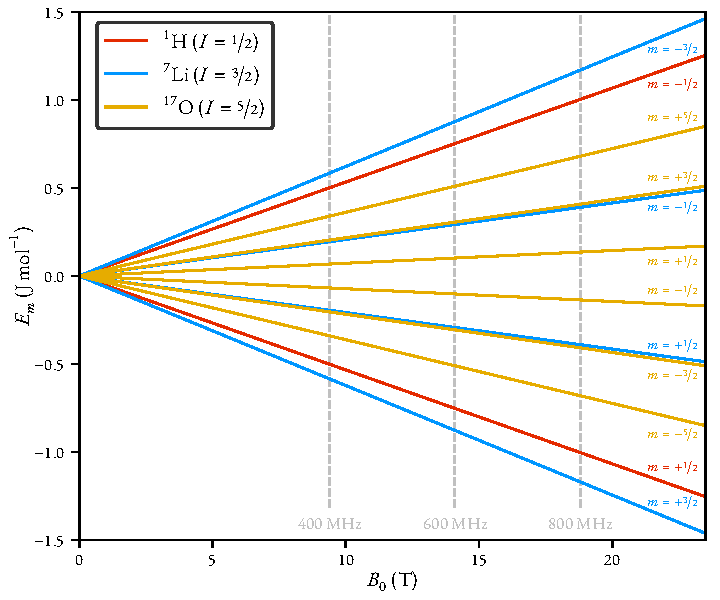
\includegraphics{energy_levels/energy_levels.pdf}%
    \caption[%
        The variation of energy of the spin states of \ch{^1H},
        \ch{^7Li}, and \ch{^{17}O} with external magnetic
        field strength.
    ]{%
        The variation of energy of the spin states of \ch{^1H},
        \ch{^7Li}, and \ch{^{17}O} with external magnetic
        field strength ($B_0$) up to \qty{23.5}{\tesla}, which is
        approximately the strength of a \qty{1}{\giga \hertz} \ac{NMR} magnet.
        Three common field strengths for commercial NMR magnets are indicated:
        \qty{9.40}{\tesla} (\qty{400}{\mega\hertz}), \qty{14.10}{\tesla}
        (\qty{600}{\mega\hertz}), and \qty{18.79}{\tesla}
        (\qty{800}{\mega\hertz}). \correction{Note the relative ordering of the spin states
        for \textsuperscript{1}H and \textsuperscript{7}Li (with positive
        $\gamma$) versus \textsuperscript{17}O (with negative  $\gamma$).}
    }%
    \label{fig:energy_levels}%
\end{figure}%
\ac{NMR} samples comprise a vast ensemble of equivalent spin systems, and it is
the macroscopic properties of the sample that are observed.
At thermal equilibrium, the various spin states will be disproportionately
populated\,---\,albeit to a meager extent due to the small
relative energies involved\,---\,in accordance with the Boltzmann
distribution, with lower energy states being more heavily populated. For
example, an ensemble of
non-interacting spin-$\nicefrac{1}{2}$ nuclei with $\gamma > 0$, such as
\ch{^1H}, will have a more populated $m = +\nicefrac{1}{2}$ (\textalpha) state,
relative to the $m = -\nicefrac{1}{2}$ (\textbeta) state.  Due to the
population imbalance, the ensemble acquires a net (bulk) magnetic moment
$\symbf{M}$, given by the sum of all the individual spin moments:
\begin{equation}
    \symbf{M} = \sum\limits_{s=1}^{S} \symbf{\mu}_s,
\end{equation}
where $S \gg 1$ is the number of spins in the ensemble.
At equilibrium, the $x$- and $y$-components of the bulk magnetisation are zero:
\begin{equation}
    \sum_{s=1}^{S} \mu_{x,s} = \sum_{s=1}^{S} \mu_{y,s} = 0,
\end{equation}
such that the bulk magnetisation is collinear with the field direction, with a
magnitude $M_0$.

\correction{
    The fractional population of the state $m$ is given by:
    \begin{equation}
        p_{m} = \frac{\exp\left(\frac{m\hbar \gamma B_0}{k_{\text{B}} T}\right)}
        {\sum\limits_{m} \exp\left(\frac{m\hbar \gamma B_0}{k_{\text{B}} T}\right)},
        \label{eq:boltzmann}
    \end{equation}
    where $k_{\text{B}}$ is the Boltzmann constant
    (\qty{1.381e-23}{\joule\per\kelvin}),
    and $T$ is the sample temperature.
    N.B. $\sum_{m=-I}^I p_m = 1$.
    Given typical values of $\gamma$ ($\approx\!\!\qty{1e8}{\per\tesla\per\second}$) and
    $B_0$ ($\approx\!\!\qty{10}{\tesla}$),
    the inequality
    $\nicefrac{m\hbar\gamma B_0}{k_{\text{B}} T} \ll 1$ can be safely assumed
    at all temperatures used in solution-state \ac{NMR}. For this reason, the
    exponential terms in \cref{eq:boltzmann} may be approximated using a Taylor
    expansion truncated at the first-order term.
    Through this, it can be shown that the magnitude of the bulk magnetisation
    is given by
\begin{subequations}
    \begin{gather}
        M_0 = \sum_{s=1}^S \mu_{z,s} = S \hbar \gamma \sum_{m=-I}^{I} m p_m
            \approx \frac{S \gamma^2 \hbar^2 B_0 I (I + 1)}{3 k_{\text{B}} T}\\
        \implies M_0(I=\nicefrac{1}{2}) \approx
            \frac{S \gamma^2 \hbar^2 B_0}{4k_{\text{B}} T},%
        \label{eq:M0}%
    \end{gather}%
\end{subequations}%
}\label{corr:high-temp}%
To maximise experiment sensitivity, it is desirable to
study nuclei with high natural abundance (affecting $S$ for a given sample
concentration), and high
gyromagnetic ratio. Along with other favourable attributes such as its ubiquity
in organic molecules, \ch{^1H} is therefore by far the most popular nucleus to
study using \ac{NMR}, at least in solution-state contexts.

The bulk magnetisation experiences a torque induced by the magnetic field, with its
evolution described by
\begin{equation}
  \frac{\mathrm{d}\symbf{M}(t)}{\mathrm{d}t} = \symbf{M}(t) \times \gamma \symbf{B}(t).
  \label{eq:M-cross-B}
\end{equation}
The essence of \ac{NMR} is to manipulate and subsequently detect the evolution
of $\symbf{M}$. Manipulation is achieved by applying short bursts of \ac{RF}
radiation known as \emph{pulses} which perturb the net magnetic field away from
$\symbf{B}_0$. The contribution to the field induced by pulses is commonly
denoted $\symbf{B}_1$, such that at any given time
\begin{equation}
    \symbf{B}(t) = \symbf{B}_0 + \symbf{B}_1(t).
\end{equation}
Whenever the magnetisation vector is not collinear with the field vector\footnote{
    The cross product of two collinear vectors is $0$, so $\symbf{M}$ remains
    fixed when it is aligned with $\symbf{B}$, as is the case at equilibrium.
}, it
\emph{precesses} about the field vector. Free precession occurs
when the magnetisation is aligned away from the $z$-axis and $\symbf{B}_1 =
\symbf{0}$, leading to
\begin{equation}
  \frac{\mathrm{d}\symbf{M}(t)}{\mathrm{d}t} =
  -\gamma B_0 ( M_y(t) \symbf{i} -M_x(t) \symbf{j} + 0 \symbf{k}),
\end{equation}
where $\lbrace \symbf{i}, \symbf{j}, \symbf{k}\rbrace \in \mathbb{R}^3$ denote the
unit vectors along the laboratory $x$-, $y$-, and $z$-axes, respectively.
Under free precession, the magnetisation rotates about the $z$-axis (i.e.
$\symbf{B}_0$) at the \emph{Larmor frequency} $\omega_0 = -\gamma
B_0$.\footnote{
    While the \ac{SI} unit of magnetic field strength is the Tesla
    (\unit{\tesla}), when referring to the field strength that a spectrometer
    operates at, it is common to use \unit{\mega\hertz} instead. This refers to
    the Larmor frequency of a reference \proton\ nucleus at the
    given field strength. For example, a \qty{500}{\mega\hertz} spectrometer
    operates at a field strength of
    $\nicefrac{2 \pi \times \qty{5e8}{\per\second}}{\qty{2.6752e8}{\radian\per\tesla\per\second}}
    \approx \qty{11.74}{\tesla}$.
    \label{fn:MHz}
}

\correction{
The most common \ac{RF} pulses used in \ac{NMR} are linearly polarised and
sinusoidally modulated. As an example, a pulse which is polarised along
the laboratory $x$-axis takes the form
\begin{equation}
    \symbf{B}_1(t) = 2 B_1 \cos(\omega_{\text{RF}} t + \phi_{\text{RF}}) \symbf{i},
    \label{eq:linear-pulse}
\end{equation}
where $B_1 \ll B_0$ is the strength of the \emph{resonant} \ac{RF} field
(\emph{vide infra}),
$\omega_{\text{RF}}$ is its angular frequency,
and $\phi_{\text{RF}}$ is its phase.
This pulse can instead be thought of as the
superposition of two circular fields, rotating with opposite senses:
\begin{equation}
    \begin{split}
        \symbf{B}_1(t) = B_1(%
                \cos(\omega_{\text{RF}} t + \phi_{\text{RF}}) \symbf{i} +
                \sin(\omega_{\text{RF}} t + \phi_{\text{RF}}) \symbf{j}
            )\\%
            + B_1(%
                \cos(\omega_{\text{RF}} t + \phi_{\text{RF}}) \symbf{i} -
                \sin(\omega_{\text{RF}} t + \phi_{\text{RF}}) \symbf{j}
            ).
    \end{split}
    \label{eq:B1}
\end{equation}
Assuming that $\lvert \omega_{\text{RF}} \rvert$ and $\lvert \omega_0 \rvert$
are close in value, the circular component which rotates with the same
sense as the spin magnetisation is said to be \emph{on resonance}. The
component which rotates with the opposite sense has a negligible effect on
the magnetisation in most circumstances.
An \ac{RF} pulse may therefore be considered to take the following form to a
high degree of accuracy:
}\label{corr:rf-pulse}
\begin{equation}
    \symbf{B}_1(t) =
        B_1\left(
            \cos(\omega_{\text{RF}} t + \phi_{\text{RF}}) \symbf{i} +
            \sin(\omega_{\text{RF}} t + \phi_{\text{RF}}) \symbf{j}
        \right),
        \label{eq:B1}
\end{equation}
A great simplification to \cref{eq:M-cross-B} is realised by
considering a frame of reference which, rather than being static, rotates at
$\omega_{\text{RF}}$, as this makes the \ac{RF} field appear to be
time-independent. This is referred to as the \emph{rotating frame}, and leads
to \cref{eq:M-cross-B} being recast as
\begin{subequations}
    \begin{gather}
        \frac{\mathrm{d}\tilde{\symbf{M}}(t)}{\mathrm{d}t} = \tilde{\symbf{M}}(t) \times \gamma \tilde{\symbf{B}}(t),\\
        \tilde{\symbf{B}}(t) =
            B_1 \cos(\phi_{\text{RF}}) \tilde{\symbf{i}} +
            B_1 \sin(\phi_{\text{RF}}) \tilde{\symbf{j}} +
            \Updelta B_0 \tilde{\symbf{k}},\\
        \Updelta B_0 = -\frac{\Omega}{\gamma},\\
        \Omega = \omega_0 - \omega_{\text{RF}},\\
        \correction{
            \tilde{\symbf{i}} = \cos(\omega_{\text{RF}} t) \symbf{i} +
                \sin(\omega_{\text{RF}} t) \symbf{j},
            }\\
        \correction{
                \tilde{\symbf{j}} = \cos(\omega_{\text{RF}} t) \symbf{j}
                - \sin(\omega_{\text{RF}} t) \symbf{i},
            }\\
        \tilde{\symbf{k}} = \symbf{k}
    \end{gather}%
    \label{eq:rot-frame}%
\end{subequations}%
The tilde has been used to distinguish quantities in the rotating frame from
their laboratory frame counterparts.
$\Omega$ is the \emph{offset} of the spin
magnetisation. When $\Omega = \qty{0}{\radian\per\second}$, the \ac{RF} field is
perfectly on resonance, and at times when it is not being applied, the
magnetisation vector appears to be static in the rotating frame.

\Cref{eq:rot-frame} implies that at times when $\tilde{\symbf{M}}$ is tilted
away from $z$-axis, and not \ac{RF} pulse is being applied, it rotate
indefinitely about the $z$-axis with a
frequency of $\Omega$. However, in reality the system is driven to re-establish
its thermal equilibrium state:
\begin{equation}
    \symbf{M}_{\text{eq}} \equiv \tilde{\symbf{M}}_{\text{eq}} = 0 \symbf{i} + 0\symbf{j} + M_0 \symbf{k}.
\end{equation}
The process by which
this occurs is called \emph{relaxation}.
\correction{
    \label{corr:relaxation}
    Spin relaxation is driven by the stochastic motion of the molecules in
    the sample, which give rise to variations in the magnetic fields
    present. The fields induced by molecular motion vary with time, and average
    to zero. Furthermore, in different locations within the sample, the
    variation in these fields with time is uncorrelated. As a result, these
    fields are often referred to as \emph{local} fields.
    The presence of time-varying local fields in the sample lead to a number of
    mechanisms that contribute to relaxation. These mechanisms are often classified
    based on whether or not they are associated with an energy transfer:
    \begin{itemize}
        \item \emph{Adiabatic interactions} do not require a transfer of energy
            between a spin system of interest and its surroundings\footnote{
                \correction{
                    The surroundings of a particular spin system of interest is
                    often referred to as the \emph{lattice}, which contains all
                    degrees of freedom in the sample other than those of the spin
                    system itself, including motional degrees of freedom of all
                    molecules in the system, and the spin energy levels of all
                    other molecules.
                }
            }. Molecular motion results in the $z$-component of the magnetic
            field experienced by a given spin to vary with time.
            The associated Larmor frequency of the spin is perturbed in
            accordance with this field variation.
            Spins in different locations, experiencing
            differing local $z$-field fluctuations, will gradually lose
            synchronisation with each other (i.e. become \emph{dephased}) as
            their instantaneous Larmor frequencies are non-equivalent. The
            effect of this is for the transverse component of the bulk
            magnetisation to decay. Hence, adiabatic interactions contribute to
            \emph{transverse relaxation}, also referred to as \emph{spin-spin
            relaxation}.
        \item \emph{Nonadiabatic interactions} involve the transfer of energy
            between a spin and its surroundings. Molecular motion which leads
            to varying transverse ($xy-$) magnetic fields with a component that
            fluctuates at the spin's Larmor frequency is able to induce such an
            energy transfer. This mechanism drives the relative populations of
            the spin's energy levels towards their equilibrium configuration,
            restoring the $z$-component of the bulk magnetisation.
            As such, nonadiabatic interactions contribute towards
            \emph{longitudinal relaxation}, also referred to as
            \emph{spin-lattice relaxation}.
            Furthermore, due to the finite lifetimes of the spin states,
            their associated energies are not perfectly defined, in accordance
            with the Heisenberg uncertainty principle. Because of this,
            nonadiabatic interactions also contribute towards transverse
            relaxation.
    \end{itemize}
    In the Bloch model, the influence of longitudinal and transverse relaxation are
    accounted for by the incorporation of two processes with respective rate
    constants $R_1$ and $R_2$ (both with units of \unit{\per\second}). These
    processes are often described in terms of relaxation times
    instead: $T_i \coloneq \nicefrac{1}{R_i}, i \in \lbrace 1, 2\rbrace$.  In
    the vast majority of situations, the rate of transverse relaxation is
    greater than that of longitudinal relaxation, i.e. $T_2 \leq
    T_1$~\cite[Section 11.9]{Levitt2007}. The rate of longitudinal relaxation
    places a strict limit on the rate of transverse relaxation: $T_2 \leq 2
    T_1$; if this were violated, during the evolution of the bulk magnetisation
    vector, its magnitude would surpass its magnitude at equilibrium, which is
    a physical impossibility~\cite{Traficante1991}.
    The introduction of relaxation is phenomenological in the Bloch model; the
    reversion of the spin system to equilibrium is included purely to ensure
    the model agrees with observation. More sophisticated theories invoking
    Liouville-space quantum mechanics can account for
    relaxation however~\parencites[Chapter 5]{Cavanagh2007}[Chapter 6]{Kuprov2023}{Goldman2001}{Kuprov2007}.
}

\begin{figure}
    \centering
    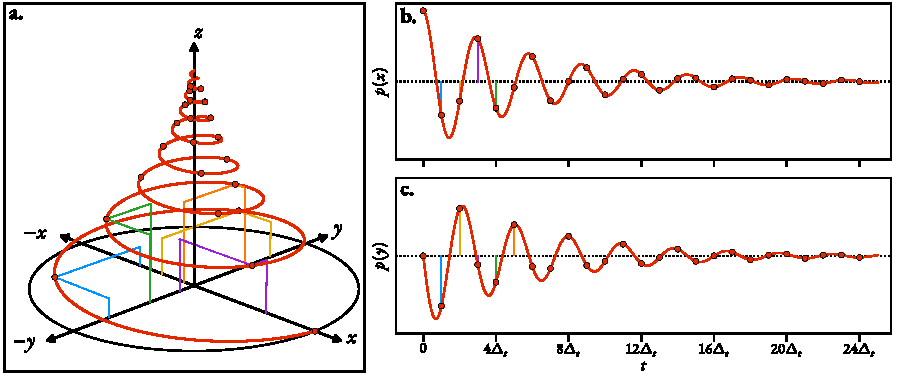
\includegraphics{quadrature_detection/quadrature_detection.pdf}
    \caption[
        The free evolution of the bulk magnetisation of an ensemble of
        spin-$\nicefrac{1}{2}$ nuclei according to the Bloch model.
    ]{
        \textbf{a.} An illustration of the free evolution of the bulk
        magnetisation of an ensemble of spin-$\nicefrac{1}{2}$ nuclei
        immediately after the application of a $\ang{90}_y$ pulse according to
        the Bloch model. The rate of transverse relaxation was set to be double
        that of longitudinal relaxation ($T_2 = \nicefrac{T_1}{2}$).
        The projections of the magnetisation vector onto the
        $x$- and  $y$-axes are plotted in panels \textbf{b.} and \textbf{c.},
        respectively. Modern \acs{NMR} spectrometers utilise quadrature
        detection, such that the $x$- and  $y$- projections of the time-varying
        magnetisation are sampled at regular time intervals, separated by
        $\Dt$.  The resulting \acs{FID} is given by the complex value $p(x) +
        \iu p(y)$.
    }\label{fig:quadrature}
\end{figure}

Everything has now been established to state the Bloch equations, which
describe the evolution of the bulk magnetisation of an ensemble of identical
spin-$\nicefrac{1}{2}$ nuclei in the rotating frame:
\begin{equation}
    \frac{\mathrm{d}\tilde{\symbf{M}}(t)}{\mathrm{d}t} =
    \begin{bmatrix}
        -R_2 & -\Omega & \omega_1 \sin(\phi_{\text{RF}}) \\
        \Omega & -R_2 & -\omega_1 \cos(\phi_{\text{RF}}) \\
        -\omega_1 \sin(\phi_{\text{RF}}) & \omega_1 \cos(\phi_{\text{RF}}) & -R_1
    \end{bmatrix}
    \tilde{\symbf{M}}(t)
    + R_1 M_0
    \begin{bmatrix}
        0 \\ 0 \\ 1
    \end{bmatrix},
\end{equation}
where $\omega_1 \coloneq -\gamma B_1$.
\Cref{fig:quadrature}.a depicts the
evolution of a bulk magnetisation vector after the application of an
\ac{RF} pulse with $\phi_{\text{RF}} = \nicefrac{\pi}{2}$, and an appropriate
combination of duration and power to induce a clockwise rotation of \ang{90}
about the $y$-axis; such a pulse is denoted $\ang{90}_{y}$.
Neglecting off-resonance effects, the magnetisation vector will land on the
$x$-axis, and evolve according to
\begin{subequations}
    \begin{gather}
        \tilde{M}_x(t) = M_0 \cos(\Omega t) \exp(-R_2 t),\\
        \tilde{M}_y(t) = M_0 \sin(\Omega t) \exp(-R_2 t),\\
        \tilde{M}_z(t) = M_0 (1 - \exp(-R_1 t)),
    \end{gather}
\end{subequations}
with $t=\qty{0}{\second}$ denoting the time that the magnetisation lands on the
$x$-axis.
During acquisition, the transverse components of the bulk magnetisation are
detected by the spectrometer probe circuitry
(Figures \ref{fig:quadrature}.b and \ref{fig:quadrature}.c), such that the
resulting signal, called the \acfi{FID}, is given by
\begin{subequations}
    \begin{gather}
        y(t) \propto \tilde{M}_+(t),\\
        \tilde{M}_+(t) = \tilde{M}_x (t) + \iu \tilde{M}_y (t) = M_0 \exp(\iu \Omega t - R_2 t).
    \end{gather}
\end{subequations}

\subsection{The NMR Spectrometer}

Modern \ac{NMR} spectrometers are capable of conducting a plethora of
experiments which can aide chemists.
In essence, a spectrometer comprises a high-field magnet, a probe, components
which are used to transmit \ac{RF} pulses to the probe, and components which
are used to process the resulting signal from the probe. A brief summary of
these is now given.

\subsubsection{The Magnet}
The static $\symbf{B}_0$ field is generated by a magnet which is composed of a
superconducting solenoid immersed in liquid helium; common materials used for
the solenoid include Nb-Ti alloy and Nb\textsubscript{3}Sn. To minimise the
extent of helium evaporation, the dewar containing the helium is lined with
a thermal radiation shield. The helium dewar is then surrounded by a larger
dewar containing liquid nitrogen,
\correction{which is finally encased in a vacuum chamber.\label{corr:vacuum}}
A bore passes through the $z$-direction of
the magnet, which is maintained at a user-specified temperature. Within the
bore sits the probe. Magnets with high field
strengths are desirable, as both the resolution ($\propto B_0$) and \ac{SNR}
($\propto B_0^{\nicefrac{3}{2}}$) of the data are affected. At the
time of writing, commercial spectrometers which operate at and above a
\ch{^1H} Larmor frequency of \qty{1}{\giga\hertz} (\qty{23.5}{\tesla}) exist,
though these are uncommon and are employed primarily for the study of large
biomolecules
\correction{and solid-state \ac{NMR}\label{corr:solid-state}}.
For most applications, including
the study of small molecules, spectrometers with more modest field strengths on
the order of \qty{100}{\mega\hertz} are typically adequate. Due to their cheap
operating costs and small size, ``benchtop'' \ac{NMR} spectrometers, which
comprise permanent magnets and typically operate on the order of
\qty{10}{\mega\hertz}, have also become popular in educational and
high-throughput settings~\cite{Giberson2021}.

To ensure a high spatial field homogeneity (a necessity for data with
acceptable resolution) a series of coils called \textit{shims} surround the
sample. Each coil produces a weak magnetic field with a specific spatial
profile in accordance with a spherical harmonic function; a collection of shims
can cancel out
\correction{small\label{corr:small-inhomog}}
inhomogeneities inherent to the main magnet~\cite[Chapter1, Appendix
B]{Webb2016}.
A field-frequency lock is used to ensure the stability of the
field. The lock is effectively a small \ac{NMR} spectrometer, tuned to a
specified isotope (typically \textsuperscript{2}H\footnote{
    \textsuperscript{2}H-enriched solvents are routinely used to make up
    \ac{NMR} samples. In \proton\ \ac{NMR} experiments, this ensures that an
    extremely intense signal due to the solvent does not dwarf the signals from
    other spins in the sample. This makes \textsuperscript{2}H a suitable
    nucleus to monitor by the lock, as it present in high concentrations, but
    rarely directly studied.
}), which monitors the resonance frequency of the isotope over
time. If the frequency begins to drift, the current in the $Z_0$ coil is
appropriately adjusted, which induces a constant change in field strength
throughout the sample volume.

\subsubsection{The Probe}
\correction{The probe sits inside the bore of the magnet and has a number of
responsibilities including holding the sample, regulating the sample temperature,
and housing the coils used to pulse the sample with \ac{RF}
radiation, as well as coils which are used to generate field
gradients\cite[Section 4.7]{Levitt2007}.\label{corr:probe}}
The \ac{RF} coils also receive the response from the sample during detection.
The principle source of data corruption in \ac{NMR} experiments is thermal
noise within the probe circuitry.  For this reason, cryogenic probes have
become a popular development, in which the coils and other probe electronics
are maintained at a very low temperature (typically about
$\qty{20}{\kelvin}$)~\cite{Kovacs2020}.

\subsubsection{The Transmitter}
The transmitter is responsible for the generation of \ac{RF} pulses
with specified power, timing and phase.
A synthesiser acts as an \ac{RF} source, producing a continuous carrier wave at
or very close to the Larmor frequency of the target nucleus. This frequency
($\omega_{\text{RF}}$) can be adjusted in order to determine the center of the
spectrum. The difference between the carrier frequency and the reference
``basic frequency'' of the spectrometer is referred to as the \emph{transmitter
offset} $\foff$.  The output of the synthesiser is gated to ensure pulses are
applied at the desired times. Attenuators/amplifiers then adjust the power
of the pulse, which travels to the probe.

\subsubsection{The Receiver}
During detection, the time-varying current induced in the probe coil by
the sample magnetisation \correction{travels to\label{corr:travel}} a receiver,
which comprises a series of components designed to convert the
analogue current to the digital \ac{FID} which is stored in computer memory.
One of the processes that the receiver is responsible for is \emph{quadrature
detection}~\cite[Section 13.6]{Keeler2010}, which ensures
\acp{FID} are frequency discriminated, i.e. that they possess the requisite
information to determine whether a given component in the \ac{FID} has a
frequency that is above or below the transmitter frequency.
This is achieved by splitting the signal from the probe into two channels. In
each channel, the signal, which is of a very high frequency
(\unit{\mega\hertz}), is mixed with a reference signal of frequency
$\omega_{\text{RF}}$. The mixing process results in a low-frequency
(\unit{\kilo\hertz}) signal being generated, along with a very high frequency
signal. The reference signal in one channel possesses a phase which
is shifted by \ang{90} relative to the other, such that the combined signal
constitutes a quadrature pair.
Both signals are then sent through a low-pass filter to remove
the high frequency component produced through mixing. Finally, an analogue to
digital converter translates the signal to the real and imaginary components of
a binary dataset which constitutes the \ac{FID}.

\subsection{The Structure of the \acs{FID}}
The result of running a \ac{1D} \ac{NMR} experiment is an \ac{FID} $\by \in
\mathbb{C}^N$ which is sampled at equally spaced points in time, with
consecutive samples separated by time $\Dt$:
\begin{equation}
    \begin{gathered}
        \by = \begin{bmatrix}
            y_0 & y_1 & y_2 & \cdots & y_{N-1}
      \end{bmatrix}\T\\
      \equiv
      \begin{bmatrix}
          y(t=0) & y(t=\Dt) & y(t=2\Dt) & \cdots & y(t=(N-1)\Dt)
      \end{bmatrix}\T,
    \end{gathered}
\end{equation}
where $y(t)$ is the (continuous) variation of the generated signal as a
function of time,
and $N$ (often a power of 2) is the number of points sampled. The inverse of
the sampling rate,
$\nicefrac{1}{\Dt}$ is the \correction{\emph{spectral width}\label{corr:sw}} $\fsw$ which
defines how large the range of samplable frequencies is, in accordance with the
Nyquist theorem~\cite{Shannon1949}.

\acp{FID} adopt the form of a summation of $M \in \mathbb{N}$ complex
exponentials; these will be referred to as \emph{signals} in this text. Each
signal will be subjected to damping due to transverse relaxation, which is
typically exponential in nature. An \ac{FID}
therefore takes the form\footnote{
    \correction{
        This provides an idealised model of an \ac{FID}, based on the
        underlying theory of the experiment. In reality, there is the possibility
        of significant deviations from this model being realised. One potential
        cause of this is the influence of magnetic field inhomogeneities, which
        will cause spectral peaks to deviate from having Lorentzian lineshapes
        (\cref{subsec:nmr-proc}). In cases where distortions to the data have
        occurred, techniques such as \emph{reference deconvolution}~\cite{Morris1997}
        can be used as a corrective measure in a bid to make the data agree more
        closely with this model.
    }\label{fn:ref-decon}
}
\begin{subequations}
    \begin{gather}
        y_n = x_n(\bth) + w_n \quad
            \quad \forall n \in \lbrace 0, 1, \cdots, N - 1 \rbrace,
            \label{eq:y=x+w} \\
        x_n(\bth) =
        \sumM \amexpphim \exp\left(
            (2 \pi \iu (f_m - \foff)- \eta_m ) n \Dt
        \right).
        \label{eq:x-1d}
    \end{gather}
    \label{eq:1d}%
\end{subequations}%
\cref{eq:1d} indicates that \iac{FID} comprises a deterministic contributions
from the evolution of the spin magnetisation $\bx$, as well as one from
experimental noise $\bw$ (\emph{vide infra}). Each signal which contributes to
$\bx$ is defined by four parameters:
\begin{itemize}
    \item Amplitude $a \in \mathbb{R}_{>0}$ ,
    \label{pg:param-constraints}
    \item Phase $\phi \in (-\pi, \pi]$ (\unit{\radian}),
    \item Frequency $f \in \left[\hspace*{2pt}\foff - \nicefrac{1}{2} \hspace*{2pt}
        \fsw, \foff + \nicefrac{1}{2} \hspace*{2pt}\fsw \right]$ (\unit{\hertz}),
    \item Damping factor $\eta \in \mathbb{R}_{>0}$ (\unit{\per\second}).
\end{itemize}%
\Iac{FID} can therefore be parameterised by the vector $\bth \in
\mathbb{R}^{4M}$:
\begin{equation}
    \bth =
    \begin{bmatrix}
        \symbf{a}\T & \symbf{\phi}\T & \symbf{f}\T & \symbf{\eta}\T
    \end{bmatrix}\T,
\end{equation}
where $\bda \in \mathbb{R}^M = [a_1 \hspace{2pt} a_2 \hspace{2pt} \cdots
\hspace{2pt} a_M]^{\mathrm{T}}$ is a vector of all amplitudes, $\bdphi \in
\mathbb{R}^M$ is a vector of all phases, etc.
A more concise alternative to \correction{\cref{eq:x-1d}}
involves the \emph{complex amplitudes} and \emph{signal poles} associated with
the \ac{FID}:
\begin{subequations}
    \begin{gather}
        x_n(\bth) = \sumM \alpha_m^{\vphantom{n}} z_m^n,\\
        \alpha_m = \amexpphim,\\
        z_m = \exp\left(
            \left(2 \pi \iu \left(f_m - \foff\right) - \eta_m\right) \Dt
        \right).\label{eq:signal-pole}
    \end{gather}
    \label{eq:x-alpha-z}%
\end{subequations}
The respective influences of the four parameters on a signal in the time-domain
are depicted in Figures \ref{fig:amp-phase-freq-damp}.a1 to
\ref{fig:amp-phase-freq-damp}.d1.
\begin{figure}
    \centering
    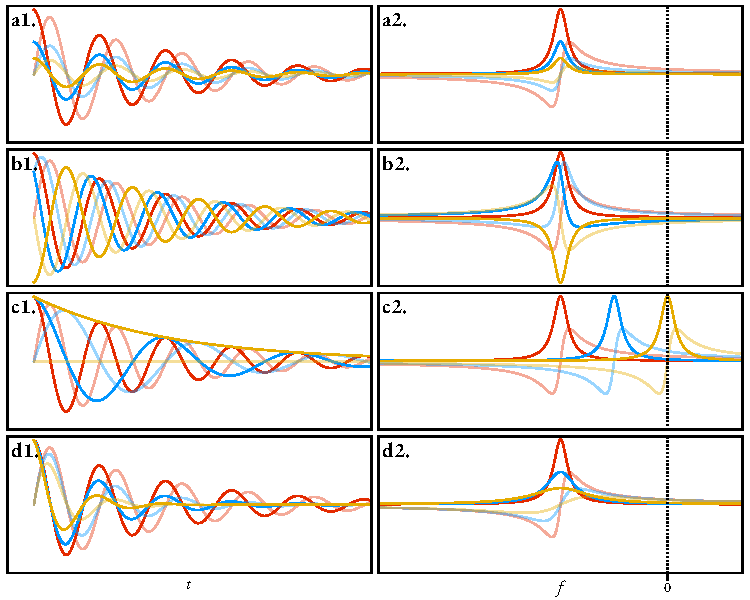
\includegraphics{amp_phase_freq_damp/amp_phase_freq_damp.pdf}
    \caption[
        The influence of the four parameters associated
        with an exponentially damped complex sinusoidal signal in both the
        time-domain and the Fourier-domain.
    ]{
        The influence of the four parameters associated
        with an exponentially damped complex sinusoidal signal in both the
        time-domain (a1 to d1) and Fourier-domain (a2 to d2).
        The red signal is generated with the same parameters across all panels:
        $a = a_{\text{red}}$, $\phi = 0\,\unit{\radian}$, $f = f_{\text{red}}$,  $\eta =
        \eta_{\text{red}}$.  The blue and yellow signals were produced by
        altering one parameter out of the four.
        \textbf{a.} $a_{\text{yellow}} = \nicefrac{1}{2} a_{\text{blue}} =
        \nicefrac{1}{4} a_{\text{red}}$.
        \textbf{b.}
        $\phi_{\text{blue}} = \nicefrac{\pi}{4}\,\unit{\radian}$,
        $\phi_{\text{yellow}} = \pi\,\unit{\radian}$.
        \textbf{c.}
        $f_{\text{blue}} = \nicefrac{1}{2} f_{\text{red}}$,
        $f_{\text{yellow}} = 0$.
        \textbf{d.}
        $\eta_{\text{yellow}} =
        \nicefrac{1}{2}\eta_{\text{blue}} =
        \nicefrac{1}{4}\eta_{\text{red}}$.
        The real and imaginary components of each signal are plotted, with the
        imaginary component being paler than its real counterpart.
    }
    \label{fig:amp-phase-freq-damp}%
\end{figure}

Multidimensional experiments~\cite[Chapter 4]{Cavanagh2007} involve
incrementing one or more delays within a
pulse sequence, in order to obtain an array of \ac{1D} \acp{FID}. In a
$D$-dimensional dataset, each contributing signal is parameterised by an
amplitude and phase as before, along with $D$ distinct frequencies and damping
factors, such that a general parameter vector  $\bth \in \mathbb{R}^{2(1+D)M}$
is given by
\begin{equation}
    \bth =
    \begin{bmatrix}
    \symbf{a}\T &
    \symbf{\phi}\T &
    {\bdfone}\T &
    \cdots &
    {\bdfD}\T &
    {\bdetaone}\T &
    \cdots &
    {\bdetaD}\T
    \end{bmatrix}\T,
    \label{eq:theta}
\end{equation}
where $\bdfD$ and $\bdetaD$ are the frequencies and damping factors in the
actively acquired (direct) dimension, and $\lbrace \bdfone, \cdots,
\bdfDminusone \rbrace$ and
$\lbrace \bdetaone, \cdots, \bdetaDminusone \rbrace$ are those of the indirect
dimension(s).
Indirect dimensions can exhibit different forms of evolution, depending on
the precise nature of the pulse sequence, of which two are very
common~\cite[Section 4.3.4]{Cavanagh2007}. \acp{FID} whose constituent signals
evolve according to $\cos(2 \pi f t)$ or $\sin(2 \pi f t)$ modulate the
amplitude of the direct dimension across increments, while those whose signals
evolve according to $\exp(2 \pi \iu f t)$ and $\exp(-2 \pi \iu f t)$ modulate
the phase instead.
For experiments which produce amplitude-modulated \acp{FID},
both the cosine and sine forms should be acquired if possible, as this ensures
that spectra with desirable properties can be generated. The same is true for the positive
and negative forms when phase-modulated \acp{FID} are acquired (\emph{vide
infra}). In general, a $D$-dimensional \ac{FID} $\bY \in \mathbb{C}^{\None
\times \cdots \times \ND}$ can be expressed as
\begin{subequations}
    \begin{gather}
        \ynonenD = \xnonenD(\bth) + \wnonenD,\\
        \xnonenD
            = \sumM \amexpphim \prodD
            \zeta^{(d)}\left(2 \pi \left(f^{(d)}_m  - \foffd\right) \nd \Dtd\right)
            \exp\left(-\eta^{(d)}_m \nd \Dtd\right),\\
        \zeta^{(d)}(\cdot)
        \begin{cases}
            = \exp(\iu\cdot) & d = D \\
            \in \left\lbrace \cos(\cdot), \sin(\cdot), \exp(\iu\cdot) \exp(-\iu\cdot)\right\rbrace & \text{otherwise}
        \end{cases}.
    \end{gather}
    \label{eq:general-fid}%
\end{subequations}%

It is typical to assume that the data is corrupted by an array of \ac{AWGN},
i.e. the noise instances are described by a complex normal distribution with
mean 0, and pairs of noise instances are statistically independent, regardless
of their time separation:
\begin{subequations}
    \begin{gather}
        \wnonenD \sim
        \mathcal{N_C}\left(0, 2\sigma^2\right) \\
        \begin{gathered}
            \implies \Re\left(\wnonenD\right) \upmodels \Im\left(\wnonenD\right),\\
             \Re\left(\wnonenD\right) \sim \mathcal{N}\left(0, \sigma^2\right),\\
             \Im\left(\wnonenD\right) \sim \mathcal{N}\left(0, \sigma^2\right). \\
        \end{gathered}
    \end{gather}
\end{subequations}
The extent by which \iac{FID} is corrupted by noise is given by its \acf{SNR}:
\begin{equation}
    \SNR\left(\bY\right) \coloneq
        \frac{1}{2 N_{\text{tot}} \sigma^2}
        \sum_{\none=0}^{\None-1} \cdots \sum_{\nd=0}^{\ND-1}
        \left \lvert \xnonenD \right \rvert^2,
        \label{eq:snr}
\end{equation}
where $N_{\text{tot}} \coloneq \None \times \cdots \times \ND$ is the total
number of points the \ac{FID} comprises. Due to the large dynamic range
observed for the \ac{SNR} across datasets, it is common to express it using a
logarithmic scale instead, in units of decibels (\unit{\deci\bel}):
\begin{equation}
    \SNR_{\unit{\deci\bel}} \coloneq 10 \log_{10} \left(\SNR\right).
    \label{eq:snr-db}
\end{equation}

\section{An Overview of NMR Data Analysis}
To gain insights from \ac{NMR} experiments on the chemical system of interest,
extraction of the defining parameters $\bth$ is necessary, though the majority
of \ac{NMR} users are unlikely to think about the process of \ac{NMR} analysis
in this way. For example:
\begin{itemize}
    \item An understanding of the chemical environments of atoms in a molecule
        can be gained by considering the chemical shifts of the various peaks
        in the spectra, which are a proxy for the \ac{FID} frequencies
        $\symbf{f}$.
    \item  The relative stoichiometries\note{does this make sense?} of a
        molecule can be elucidated by inspecting the integrals of spectral
        peaks, which are directly related to the \ac{FID} amplitudes $\bda$
\end{itemize}

\note{
    \begin{itemize}
        \item Typical approach to analysing the data (FT, peak pick, integrate, baseline correction, window functions, zero-filling etc),
        \item Estimation techniques: LP, SVD techniques, iterative techniques (AMARES, VARPRO), Bayesian techniques (CRAFT), ML techniques
    \end{itemize}
}

\subsection{Conventional NMR Analysis}
\label{subsec:nmr-analysis}
The conventional route to interpret \ac{NMR} experiments is to
transform the \ac{FID} into the frequency domain, producing an
\ac{NMR} spectrum. This is achieved through application of the \acfi{FT}:
\begin{subequations}
    \begin{align}
        &\text{Continuous case:} &&\FT(x(t))(F) =  \int_{0}^{\infty} x(t) \exp(
            -2 \pi \iu t F
            ) \mathrm{d} t
            \quad \forall t \in \mathbb{R},\\
        &\text{Discrete case:} &&\FT( \symbf{x} )_n =  \sum_{k=0}^{N-1} x_k \exp \left(
            -\frac{2 \pi \iu k n}{N} \right)
            \quad \forall n \in \lbrace 0, \cdots, N-1 \rbrace.
    \end{align}
\end{subequations}
The \ac{FT} of a continuous exponentially-damped complex sinusoid
takes the form of a \emph{Lorentzian}\footnote{
    An upshot of only possessing data for $t \geq 0$ is
    that the \ac{FT} of an \ac{FID} features a vertical offset,
    such that the baseline does not sit at 0\cite{Tang1994}. This is corrected
    by halving the initial point of the \ac{FID} prior to \ac{FT}.
}:
\begin{subequations}
    \begin{gather}
        s(F) = \FT\left(
            a \exp(\iu \phi) \exp((2 \pi \iu f - \eta)t)
            \right)(F),\\
        s(F) = \frac{a \exp(\iu \phi) }
            {\eta + 2 \pi \iu (f - F)}.
    \end{gather}
\end{subequations}
When $a = \phi = 0$, this function is equivalent to the (unnormalised) \ac{pdf}
of the Cauchy distribution. The \ac{FT} is a linear function, such that the
\ac{FT} of a summation of signals is equivalent to the summation of the
\acp{FT} of each signal. A corollary is that an \ac{NMR} spectrum comprises a
series of Lorentzian ``peaks'', located at the frequencies of all the signals
in the \ac{FID}:
\begin{equation}
    s\left(F\right) = \sum_{m=1}^{M}
    \frac{\amexpphim}
    {\eta_m + 2 \pi \iu (f_m - F)}.
    \label{eq:ft-summation}
\end{equation}
The \ac{FT} is a very attractive means of processing \ac{NMR} data, as it
presents the data in a format which is human-interpretable, with the basic
rules describing how chemical structure is mapped to \ac{NMR} spectral
properties being a fundamental skill that virtually all experimental chemists
require\cite{Hore2015b}. Due to innate properties of the \ac{NMR} experiment,
as well as features arising from analysing a discrete signal, the raw output
from an \ac{NMR} experiment often leads to spectra with undesirable
characteristics without any extra manipulation. Extra processing
steps that are frequently applied to \ac{NMR} data are now outlined, in the
order that they are applied to the data. Note that apodisation and zero filling
are applied to the \ac{FID} (prior to \ac{FT}), while phase correction and
baseline correction are applied to the spectrum (after \ac{FT}).

\begin{figure}
    \centering
    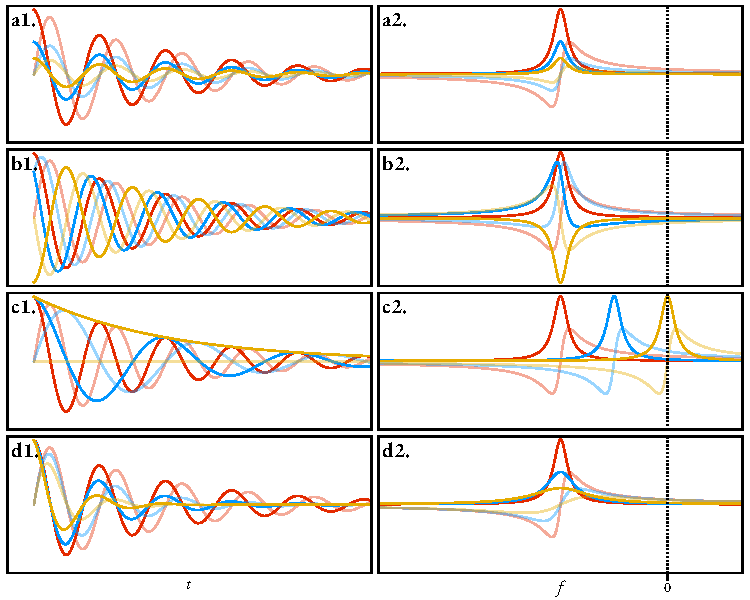
\includegraphics{amp_phase_freq_damp/amp_phase_freq_damp.pdf}
    \caption[
        An illustration of the influence of the four parameters associated
        with an oscillator in both the time-domain nels and Fourier-domain.
    ]{
        An illustration of the influence of the four parameters associated
        with an oscillator in both the time-domain (panels \textbf{a1.} --
        \textbf{d1.}) and Fourier-domain (panels \textbf{a2.} -- \textbf{d2.}).
        The red signal is generated with the same parameters across all panels:
        $a = a_{\text{red}}$, $\phi = 0$, $f = f_{\text{red}}$,  $\eta =
        \eta_{\text{red}}$.  The blue and yellow signals were produced by
        altering one parameter out of the four.
        \textbf{a.} $a_{\text{yellow}} = \nicefrac{1}{2} a_{\text{blue}} =
        \nicefrac{1}{4} a_{\text{red}}$.
        \textbf{b.}
        $\phi_{\text{blue}} = \nicefrac{\pi}{4}$,
        $\phi_{\text{yellow}} = \pi$.
        \textbf{c.}
        $f_{\text{blue}} = \nicefrac{1}{2} f_{\text{red}}$,
        $f_{\text{yellow}} = 0$.
        \textbf{d.}
        $\eta_{\text{blue}} = \nicefrac{1}{2}\eta_{\text{red}}$,
        $\eta_{\text{yellow}} = \nicefrac{1}{4}\eta_{\text{red}}$.
        The real and imaginary components of each signal are plotted, with the
        imaginary component being paler than its real counterpart.
    }
    \label{fig:amp-phase-freq-damp}
\end{figure}

\subsubsection{Apodisation}
Apodisation refers to the process of mutating a signal by multiplying it with a
specified function, often called a \emph{window function}, in order to enhance
a certain property. Apodisation is employed to improve either the sensitivity
or the resolution of the final spectrum, albeit at the cost of worsening the
other feature. There is no such thing as a free lunch after all.

\paragraph{Sensitivity Enhancement} As \iac{FID} progresses with time, the
contributions from the desirable signal ($\bx$) and experimental noise ($\bw$)
becomes more
weighted towards the noise, as spin relaxation phenomena dampen the signal. As
such, multiplying the \ac{FID} with a function which is initially large and
gets progressively smaller with time can be used to enhance the \ac{SNR} of the
\ac{FID}. The most common function to achieve this is the negative exponential
such that a given point is multiplied by $\exp(-\nicefrac{k n}{N - 1})$.
$k$ is referred to as the line broadening factor, since the increased dampening
applied to the signal causes the linewidth of the spectral peaks to increase
(see panel d of Figure \ref{fig:amp-phase-freq-damp}). As such, peaks become
more poorly resolved.

\paragraph{Resolution Enhancement} By contrast, resolution enhancement can be
achieved by applying a window function that artificially reduces the rate of
oscillator decay, by suppressing points that are early in the \ac{FID}. Popular
examples of window functions for resolution enhancement are the Lorentz-Gauss
function, which bestow a sharper, Gaussian shape to the peaks, and the
sine-bell, which is commonly used in multidimensional experiments. Since the
initial points in the \ac{FID} are attenuated these window functions reduce the
sensitivity of the resulting spectra.

By being defined to decay to a sufficiently small value, or $0$, at the end of
the \ac{FID}, window functions are also able to suppress \emph{truncation
artefacts}, which appear when the \ac{FID} still possesses appreciable signal
amplitude at the end of the acquisition period. Truncated \acp{FID} produce
spectra with peaks of a form that is akin to the convolution of the \ac{FT} of
the untruncated \ac{FID}, with the \ac{FT} of a box-function, which takes the
form of a sinc function ($\nicefrac{\sin(x)}{x}$). The resulting artefacts in
spectra are often referred to as \emph{sinc wiggles} for this reason.

\subsubsection{Zero filling}
\note{TODO}

\subsubsection{Phase correction}
The real and imaginary components of \eqref{eq:ft-summation} are as follows:
\begin{subequations}
    \begin{gather}
        \Re(s(F)) = \sum_m
        a_m (\cos(\phi_m) \mathcal{A}_m(F) + \sin(\phi_m) \mathcal{D}_m(F)),\\
        \Im(s(F)) = \sum_m
        a_m (\sin(\phi_m) \mathcal{A}_m(F) - \cos(\phi_m) \mathcal{D}_m(F)),
    \end{gather}
\end{subequations}
where $\mathcal{A}_m$ and  $\mathcal{D}_m$ denote \emph{absorption} and
\emph{dispersion} Lorentzians, respectively:
\begin{subequations}
    \begin{gather}
        \mathcal{A}_m(F) = \frac{\eta_m}{\eta_m^2 + 4 \pi^2 (f_m - F)^2},\\
        \mathcal{D}_m(F) = \frac{2 \pi (f_m - F)}{\eta_m^2 + 4 \pi^2 (f_m - F)^2}.
    \end{gather}
\end{subequations}
As illustrated most clearly in panel c2 of Figure
\ref{fig:amp-phase-freq-damp}, a peak with an absorption lineshape is far more
desirable than one with a dispersion lineshape for two key
reasons: (a) its maximum corresponds to the oscillator frequency, while a
dispersion Lorentzian has a magnitude of $0$ at the oscillator frequency (b)
they decay more rapidly towards $0$ and are therefore more resolved. Generating
a spectrum where all peaks possess absorption Lorentzians is therefore desired,
which is possible if all signal have a phase of \ang{0}, which leads to
\begin{subequations}
    \begin{gather}
        \Re(s(F)) = \sum_m a_m \mathcal{A}_m(F),\label{eq:absorption}\\
        \Im(s(F)) = -\sum_m a_m \mathcal{D}_m(F).\label{eq:dispersion}
    \end{gather}
\end{subequations}
 Fortunately, for the majority of \ac{NMR} experiments\footnote{
     An example of an exception to this rule is when \acl{FS} pulses are applied,
     which generate datasets with quadratic phase behaviour. This is discussed
     in more detail in Section \ref{sec:bbqchili}.
}, the contributing signals possess phases which depend linearly on their
frequencies, i.e.
\begin{equation}
    \phi_m = \Phi_0 + \Phi_1 f_m,
\end{equation}
where $\Phi_0, \in (-\pi, \pi]$ and $\Phi_1 \in \mathbb{R}$ are zero- and
first-order phase terms. A feature of all \ac{NMR} processing platforms is the
ability to perform phase-correction, in which the user determines
$\Phi_0$ and $\Phi_1$ by inspecting the appearance of the spectrum
$\symbf{s}_{\phi}$ for different values of $p_0$ and  $p_1$, according to
\begin{equation}
    s_{\phi,n} = s_n
    \exp\left(\iu \left(p_0 + \frac{p_1 n}{N - 1}\right)\right),
\end{equation}
in an attempt to give all peaks in the spectrum absorption-mode lineshapes.

\subsubsection{Baseline correction}
The \emph{baseline} of an \ac{NMR} spectrum is used to describe regions where
no discernible peaks reside (i.e. only experimental noise exists).
Baseline distortion is used to describe scenarios when the baseline, rather
than exhibiting a flat profile with a moving average of zero, has a distorted
shape instead. There a number of potential causes of baseline distortion,
including acquisition starting at a time $\neq 0$, ``clipping'' of the initial
points due to excessive receiver gain, and ``baseline roll'' due to the
transient response of audio filters\parencites[Section~3.3]{Cavanagh2007}{Tang1994}.
Whatever the cause(s), it is typically the corruption of the initial points in the
\ac{FID} that causes baseline distortion.
It is common to apply baseline correction algorithm after phase correction has
been undertaken to negate any distortion. This involves multiplying
the spectrum with a high-order polynomial function, whose coefficients are
determined by an appropriate algorithm. A popular algorithm
involves the two-step procedure of (a) determining spectral regions which are
part of the baseline (b) fitting the baseline regions to a
polynomial\cite{Dietrich1991,Cobas2006}.

\subsection{Conventional analysis for multidimensional datasets}
\label{subsec:mulitdim}
As for \ac{1D} datasets, it is desirable that multidimensional \ac{NMR} spectra
feature peaks which are (a) frequency discriminated, and (b) comprise pure
absorption-mode lineshapes, in each dimension. Frequency discrimination describes
the ability to determine whether a particular resonance is at a frequency which
higher or lower than the frequency of the transmitter, which is in the middle
of the spectral window. As an illustration of how this can be achieved, \ac{2D}
signals comprising a single oscillator will be considered, with
amplitude $a = 1$,  phase $\phi = \ang{0}$, frequencies $\fone$ and $\ftwo$, and
damping factors $\etaone$ and  $\etatwo$.

\subsubsection{Amplitude-modulated signals}
It is clear that a cosine modulated signal, given by \eqref{eq:general-fid}
with $D=2$ and $\zeta^{(1)} = \cos(\cdot)$ cannot achieve frequency
discrimination, on account of the relation
\begin{equation}
    \cos\left(2 \pi \fone \tone\right) =
    \tfrac{1}{2} \left(\exp\left(2 \pi \iu \fone \tone \right) + \exp\left(-2 \pi \iu
    \fone \tone \right)\right)
\end{equation}
\ac{FT} of a cosine-modulated \ac{FID} in both dimensions leads to a spectrum
whose real component comprises two peaks, one at the true resonance frequency
$\left(\fone, \ftwo\right)$, and the other at the mirror-image frequency in the
indirect dimension, $(2\foffone - \fone, \ftwo)$. On top of this, the
peaks possess a mixture of absorption and dispersion character, with the
resultant peak shape often referred to as \emph{phase twist}\cite{Keeler1985}.
A spectrum of this form is presented in panel a of Figure \ref{fig:2d-lineshapes}.
It is possible to generate pure absorption peaks by applying \ac{FT} in the
direct dimension, setting the imaginary component to zero, and finally
applying \ac{FT} in the indirect dimension. The real component of the result
(panel b) is referred to as a \emph{double absorption} spectrum.

To achieve frequency discrimination, it is necessary to also possess the
analogous sine-modulated signal, for which $\zeta^{(1)} = \sin(\cdot)$, as this
in effect achieves quadrature detection in the indirect dimension. For
numerous multidimensional experiments, this can be achieved by repeating the
pulse sequence, with careful adjustments to the phases of particular pulses, in
a process referred to as \emph{phase cycling}\cite[Chapter 11]{Keeler2010}.
Applying the same processing as that which achieved the double absorption
spectrum for the cosine-modulated case generates a spectrum whose imaginary
component features two peaks, but with opposite signs (panel c) which is borne
out of the sine function being odd. It then becomes possible to generate a
frequency discriminated spectrum by subtracting the sine spectrum from the
cosine spectrum (panel d).

\begin{figure}
    \centering
    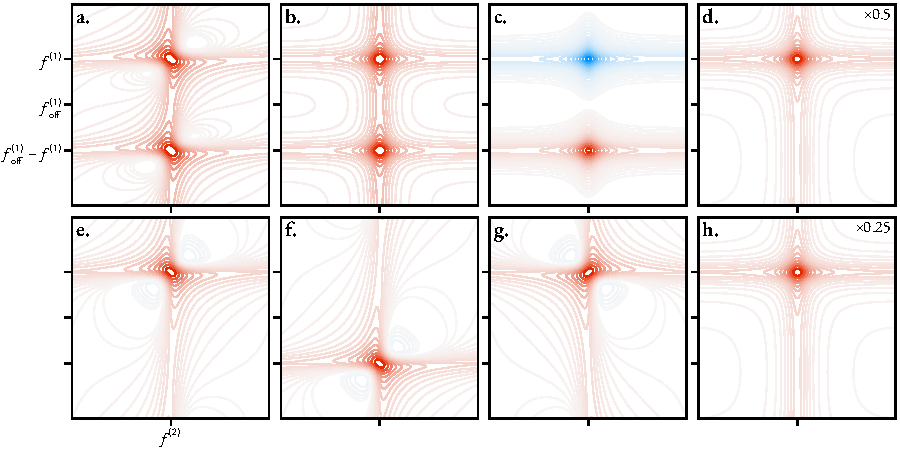
\includegraphics{2d_lineshapes/2d_lineshapes.pdf}
    \caption[
        Spectra acquired from amplitude- and phase-modulated \acs{2D} signals.
    ]{
        Spectra acquired from amplitude- and phase- modulated \acs{2D} signals.
        Red contour lines denote positive values, while blue contours denote
        negative values.
        \textbf{a.} The \ac{FT} of a cosine-modulated \ac{FID}, featuring peaks
        both at the true resonance frequency ($\fone$) and the mirrored
        frequency ($2\foffone - \fone_{\vphantom{off}}$), and with phase-twist lineshapes.
        \textbf{b.} Double-absorption spectrum generated by applying \ac{FT}
        in the direct dimension, setting the imaginary component to zero,
        applying \ac{FT} in the indirect dimension, and retaining the real
        component.
        \textbf{c.} Spectrum acquired with the same processing method as in
        \textbf{b.} but with a sine-modulated \ac{FID}, and with the imaginary
        component retained.
        \textbf{d.} The subtraction of the spectrum in \textbf{c.} from that in
        \textbf{b.} leads to a spectrum with frequency discrimination and a
        pure absorption lineshape.
        \textbf{e.} The \ac{FT} of a positive phase-modulated \ac{FID},
        exhibiting frequency discrimination, but with a phase twist shape.
        \textbf{f.} The \ac{FT} of a negative phase-modulated \ac{FID}.
        \textbf{g.} The spectrum in \textbf{f.} inverted along the indirect
        axis, about $\foffone$.
        \textbf{h.} The summation of \textbf{e.} and \textbf{g.} generates a
        spectrum with an absorption lineshape.
    }
    \label{fig:2d-lineshapes}
\end{figure}

\subsubsection{Phase-modulated signals}

A ``positive'' phase-modulated signal with the form $\zeta^{(1)} = \exp(\iu \cdot)$
(commonly referred to as \emph{hypercomplex}) is frequency-discriminated due to
its quadrature nature. However, direct \ac{FT} of such a signal in both
dimensions leads to a peaks with a phase-twist lineshape, with no means of
separating the absorption and dispersion contributions (panel e). Certain pulse
sequences, including \ac{2DJ} spectroscopy\cite{Aue1976,Morris2009} (see
Chapter \ref{chap:cupid}) and
\ac{COSY}\cite{Jeener1971,Jeener2016,Aue1976a} produce hypercomplex datasets,
and the conventional means of processing is simply to display the absolute
value of the spectrum, which while removing the phase twist shapes, produces
peaks with broad wings, due to the influence of the dispersive components. In
scenarios where it is possible, it is desirable to acquire the equivalent
``negative'' signal ($\zeta^{(1)} = \exp(-\iu \cdot)$), whose \ac{FT} leads to
a peak with the same phase twist form, but centered at $2\foffone - \fone$
(panel f). Inverting this spectrum in $\Fone$ (panel g), and summing with the
positive spectrum nullifies the dispersive contributions, generating a spectrum
with absorption lineshapes\cite{Davis1992} (panel h).

\subsection{Estimation Techniques for NMR Analysis}

\subsubsection{\Acl{LP}}

\Ac{LP}\cite{Stephenson1988,Koehl1999} is a procedure which is now widely used
in \ac{NMR} data analysis, often with the intention of (a) propagating the
\ac{FID} further in time in order to reduce the presence of truncation
artefacts and (b) correct the commonly corrupted initial points of the
\ac{FID}, as a means of improving the spectral baseline. The concept of \ac{LP}
stems from the idea that a deterministic signal, such as a \ac{1D} \ac{FID} can
be described as an \ac{AR} process, such that a given sample from the dataset
can be described by a linear combination of a certain number of previous
samples:
\begin{equation}
    \by \left[\none\right] = \sum_{l=0}^{L-1}
    \symbf{c}[l] \hspace{2pt} \by \left[ \none - l - 1\right] + \symbf{e} [l]
    \label{eq:forward-lp}
\end{equation}
$\forall \none \in \lbrace L, L + 1, \cdots, \None - 1 \rbrace$, where $L \in
\mathbb{Z}$ defines the order of the linear estimator, and $\symbf{c} \in
\mathbb{R}^{L}$ is a set of \emph{forward} \ac{LP} coefficients. $\symbf{e} \in
\mathbb{R}^L$ is a set of parameters, sometimes called the innovations, which
account of error in the \ac{LP} model. A datapoint can also be described by a
linear combination of a certain number of subsequent points, using the set of
\emph{backward} \ac{LP} coefficients $\symbf{b} \in \mathbb{R}^L$:
\begin{equation}
    \by \left[\none\right] = \sum_{l=0}^{L-1}
    \symbf{b}[l] \hspace{2pt} \by \left[ \none + l + 1\right] + \symbf{e} [l]
    \label{eq:backward-lp}
\end{equation}
$\forall \none \in \lbrace 0, 1, \cdots, \None - L - 1 \rbrace$. Determining
the \ac{LP} coefficients enables the estimation of \ac{FID} values beyond the
data actually acquired ($\none < 0$ and $\none > \None - 1$). It should be noted that
\eqref{eq:forward-lp} and \eqref{eq:backward-lp} are only valid for
\acp{FID} without any corruption from experimental noise. Noisy datasets are
instead an example of an \ac{ARMA} process. Despite this, due to the greater
simplicity of the \ac{AR} model, it is far more common to employ this. The most
common means of performing \ac{LP} is by solving the Yule-Walker
equations\cite{Yule1927,Walker1931},
which describe the relationship between the signal autocorrelation coefficients
and the \ac{LP} coefficients\cite[Section 3.3]{Koehl1999}, with the
Levinson-Durbin algorithm providing an efficient means of solving the
equations\cite{Levinson1946,Durbin1960}.

\note{Stuff below here has been copy-pasted from old document. Will need editing!}
\subsubsection{Signal-Noise Subspace Separation Techniques}

The Linear Prediction with Singular-Value Decomposition was proposed by Kumaresan and Tufts\cite{Kumaresan1982}. The core assumption of the method is that a given data point $y_n$ may be expressed as a linear combination of $L$ previous, or preceeding points:
\begin{equation}
  \begin{split}
    y_n &= b_1 y_{n+1} + b_2 y_{n+2} + \cdots + b_L y_{n+L}\\
    &= b_{-1} y_{n-1} + b_{-2} y_{n-2} + \cdots + b_{-L} y_{n-L}
  \end{split}
\end{equation}
where $b_l$($b_{-l}$), $\ l \in \{ 1, 2, \cdots, L \}$ are the backward(forward) prediction coeffiecients. For the backward prediction case, consider the follwing set of linear equations $\symbf{A} \symbf{b} = - \symbf{h}$:
\begin{equation}
  \label{lineqs}
  \begin{bmatrix}
    y_1^* & y_2^* & \cdots & y_L^*\\
    y_2^* & y_3^* & \cdots & y_{L+1}^*\\
    \vdots & \vdots & \ddots & \vdots\\
    y_{N-L}^* & y_{N-L+1}^* & \cdots & y_{N-1}^*\\
  \end{bmatrix}
  \begin{bmatrix}
    b_1\\
    b_2\\
    \vdots\\
    b_L
  \end{bmatrix}
  = -
  \begin{bmatrix}
    y_0^*\\
    y_1^*\\
    \vdots\\
    y_{N-L-1}^*
  \end{bmatrix}
\end{equation}
This equation can be augmented into the form $\symbf{A}^{\prime} \symbf{b}^{\prime} = \symbf{0}$, with $\symbf{A}^{\prime} = \left[ \symbf{h} \vert \symbf{A} \right]$ and $\symbf{b}^{\prime} = \left[1, \symbf{b}^{\mathrm{T}} \right]^{\mathrm{T}}$. For the noiseless data case (i.e. $y_n = x_n$), any row of $\symbf{A}^{\prime}$ can be written as the linear combination of $J$ linearly independent vectors $\symbf{f}_j,\ j \in \{1, 2, \cdots, J\}$\cite{Kumaresan1983}:
\begin{equation}
  \symbf{f}_j = \left[ 1, z_j^*, \left(z_j^2\right)^*, \cdots, \left(z_j^L\right)^* \right],
\end{equation}
meaning that the rank of $\symbf{A}^{\prime}$ is $J$, provided it posseses at least $J$ rows ($J \leqslant N - L$). The fact that $\symbf{b}^{\prime}$ lies in the null space of $\symbf{A}^{\prime}$ implies that $\symbf{f}_j \symbf{b}^{\prime} = 0$, such that the following holds:
\begin{equation}
  \label{lincom}
  1 + b_1 z_j^* + b_2 \left(z_j^2\right)^* + \cdots + b_L \left(z_j^L\right)^* = 0
\end{equation}
It should be noted that $L$ must satisfy $L \geqslant J$ to ensure the null space of $\symbf{A}^{\prime}$ has at least a dimension of 1.
Eqn. \ref{lincom} leads to a means of deriving the signal poles $z_j$ via polynomial $B(\zeta)$:
\begin{equation}
  B(\zeta) = 1 + b_1 \zeta^{-1} + b_2 \zeta^{-2} + \cdots + b_L \zeta^{-L},
\end{equation}
the zeros of which will occur whenever $\zeta = \left(z_j^{-1}\right)^*,\ j \in \{1, 2, \cdots, J\}$.

Of course, the prediction coefficient vector $\symbf{b}$ still needs to be determined. Eqn. \ref{lineqs} implies that the optimal vector can be determined by simple linear lest squares:
\begin{equation}
  \hat{\symbf{b}} = - \mathbf{A}^+ \symbf{h}.
\end{equation}
However, noise components of the signal will be incorporated into the solution of $\symbf{b}$. To avoid this, $\symbf{A}$ is moved from the signal-noise subspace to the signal subspace via filtration using Singular-Valued Decomposition:
\begin{equation}
  \symbf{A} = \symbf{U}
  \begin{bmatrix}
    \symbf{\Sigma}\\
    \symbf{0}
  \end{bmatrix}
  \symbf{V}^{\dagger} = \sum_{l=1}^R \sigma_l^{\vphantom{\dagger}} \symbf{u}_l^{\vphantom{\dagger}} \symbf{v}_l^{\dagger}
\end{equation}
where $R = \\mathrm{rank}(\symbf{A}) = \min(L, N)$. The matrix $\tilde{\symbf{A}}$ of rank $J$ with the closest relationship to $\symbf{A}$ is a Frobenius norm sense is given by\cite{Cadzow1988}:
\begin{equation}
  \tilde{\symbf{A}} = \sum_{l=1}^J \sigma_l^{\vphantom{\dagger}} \symbf{u}_l^{\vphantom{\dagger}} \symbf{v}_l^{\dagger}.
\end{equation}
Using the following relationship between a matrix's pseudoinverse and its SVD:
\begin{equation}
  \symbf{A}^+ = \symbf{V}
  \begin{bmatrix}
    \symbf{\Sigma}^+\\
    \symbf{0}
  \end{bmatrix}
  \symbf{U}^{\dagger},
\end{equation}
The optimal vector of prediction coeffiecients is determined by:
\begin{equation}
  \hat{\symbf{b}} = - \tilde{\symbf{A}}^+ \symbf{h} = - \sum_{l=1}^J \sigma_l^{-1 \vphantom{\dagger}} \symbf{v}_l^{\vphantom{\dagger}} \left[ \symbf{u}_l^{\dagger} \symbf{h} \right]
\end{equation}
Application: \cite{Barkhuijsen1985}

\note{HSVD, MPM, only gloss over MPM as it is described in detail in Chapter 2}

\subsubsection{Iterative Methods}

The \ac{VARPRO} method is an iterative approach to parameter estimation, developed by Golub and Pereyra\cite{Golub1973}, and applied to NMR signal analysis by van der Veen et al.\cite{VanDerVeen1988}. It relies on minimising the following quantity:
\begin{equation}
  \label{VARPRO_min}
  \hat{\symbf{\theta}} = \argmin_{\symbf{\theta}} \left \lVert \symbf{y} - \symbf{x}(\symbf{\theta}) \right \rVert^2
\end{equation}
The vector $\symbf{x}$ can be expressed in the following format:
\begin{equation}
  \label{VARPRO_Za}
  \symbf{x} =
  \begin{bmatrix}
    z_1^0 & z_2^0 & \cdots & z_J^0\\
    z_1^1 & z_2^1 & \cdots & z_J^1\\
    \vdots & \vdots & \ddots & \vdots\\
    z_1^{N-1} & z_2^{N-1} & \cdots & z_J^{N-1}\\
  \end{bmatrix}
  \begin{bmatrix}
    \alpha_1\\
    \alpha_2\\
    \vdots\\
    \alpha_J
  \end{bmatrix}
  = \symbf{Z}\symbf{\alpha}
\end{equation}
Using Eq. \ref{VARPRO_Za}, Eq. \ref{VARPRO_min} can be re-written as follows:
\begin{equation}
    \hat{\symbf{\theta}} = \argmin_{\symbf{\theta}} \left \lVert \symbf{y} - \symbf{Z}\symbf{\alpha} \right \rVert^2
\end{equation}
The complex amplitudes can be determined analytically as follows:
\begin{equation}
  \label{VARPRO_alpha}
  \hat{\symbf{\alpha}} \approx \left( \symbf{Z}^{\dagger} \symbf{Z} \right)^{-1} \symbf{Z}^{\dagger} \symbf{y} \equiv \symbf{Z}^+ \symbf{y}
\end{equation}
$\symbf{Z}^+$ is the Moore-Penrose pseudoinverse of matrix $\symbf{Z}$\cite{Penrose1955, Strang2018}. The VARPRO method determines the frequencies and damping factors via an iterative minimisation of:
\begin{equation}
  \hat{\left[\symbf{f}^{\mathrm{T}}, \symbf{\eta}^{\mathrm{T}}\right]}^{\mathrm{T}} = \argmin_{\left[\symbf{f}^{\mathrm{T}}, \symbf{\eta}^{\mathrm{T}}\right]} \left \lVert \symbf{y} - \symbf{Z}\symbf{Z}^+\symbf{y} \right \rVert^2
\end{equation}
which is achieved using the Levenberg–Marquardt algorithm\cite{Levenberg1944, Marquardt1963}. The amplitudes and phases are subsequently determined using Eq. \ref{VARPRO_alpha}. This means that the amplitudes and phases do not need initial guesses assocaited with them. Further specifications can be applied to the algorithm, reflecting the spectroscopist's knowledge of the signal under inspection. For example, if it is known that a certain set of resonances constitute a multiplet, the relative frequency differences and amplitudes will be known.

\ac{AMARES}\cite{Vanhamme1997}


\subsubsection{Bayesian Methods}
\ac{CRAFT}\cite{Krishnamurthy2013}
2D\cite{Krishnamurthy2017}
perspective\cite{Krishnamurthy2021}

\subsubsection{Machine Learning Methods}
\cite{Schmid2023}

\section{Overview of this work}

\subsection{Conception and motivation}
The central focus of this work is the development of a routine which performs
parametric estimation on \ac{NMR} datasets.
Motivation initially came from discussions within the NMR
Methodology Group in Manchester involving
Dr Mohammadali Foroozandeh and co-workers (notably Prof.  Gareth Morris and
Prof. Mathias Nilsson) while Dr Foroozandeh was a
Postdoctoral researcher there. The group were interested in generating pure
shift \ac{NMR} spectra from \ac{2DJ} datasets via appropriate post-processing
of the data.  While little progress was made when Dr Foroozandeh was based in
Manchester, he wished to continue with the project after moving to Oxford to
take up a research fellowship; I took the reins of the project when I joined
his nascent research group as a PhD student.

To ensure its applicability to \ac{2DJ} datasets, the following properties were
sought while devising what a suitable estimation routine would entail:

\paragraph{Support for \ac{1D} and \ac{2D} data}
The method should be able to analyse both \ac{1D} \acp{FID} and also
hypercomplex \ac{2D} \acp{FID} (the form which \ac{2DJ} datasets take).
\ac{2D} data should be analysed holistically,
rather than as successive \ac{1D} increments, as is the case in methods like
\ac{CRAFT}\cite{Krishnamurthy2017} and other previous approaches which will be
discussed later. This is since better signal resolution is often available when
both dimensions are considered at the same time; certain signals which exhibit
clear resolution in a \ac{2D} dataset may be heavily overlapping in \ac{1D}
data and are therefore more challenging if not impossible to quantify
accurately.

\paragraph{Time-domain based}
As discussed in \cref{subsec:multidim}, due to the hypercomplex nature of
\ac{2DJ} \acp{FID}, generating spectra with desirable absorption lineshapes is
not possible. Typically, resorting to displaying the spectra in magnitude-mode is
deemed optimal, as this overcomes the phase-twist peak lineshapes. However,
such spectra suffer from severe non-linearities and dispersion-mode
contributions, both of which make the task of estimating \ac{2DJ} data in the
Fourier domain challenging. For this reason, estimating the dataset by
considering its \ac{FID} rather than its spectrum is preferred.

\paragraph{Accessibility}
To achieve wide-spread adoption, especially by non-expert \ac{NMR} users,
the method should require minimal user intervention to perform effectively. As
such, a method requiring the specification of as little prior knowledge
about the data as possible is desired.
On top of this, the method should be available as software that users can gain
familiarity with easily.

\subsection{Thesis Overview}
The remainder of this thesis comprises the following chapters:
\begin{itemize}
    \item \textbf{\cref{chap:theory}} discusses the theory behind routines
        which can be applied to determine parameter estimates related to
        \ac{1D} and \ac{2D} \acp{FID}.
    \item \textbf{\cref{chap:results}} provides illustrations of the
        performance of the estimation routine on \ac{1D} \ac{NMR} datasets.
        Furthermore, means in which parametric estimation routine can be
        harnessed for two applications are explored:
        \begin{itemize}
            \item The analysis of amplitude-attenuated datasets, such as those
                derived from diffusion-, $T_1$- and $T_2$-measuring
                experiments (\cref{sec:seq}).
            \item Overcoming quadratic phase behaviour and baseline distortions
                associated with ultra-broadband excitation by a single
                \acl{FS} pulse (\cref{sec:bbqchili}).
        \end{itemize}
    \item \textbf{\cref{chap:cupid}} outlines a devised method, given the acronym
        \acs{CUPID}, for generating pure shift spectra from the estimation of
        \ac{2DJ} datasets.
    \item \textbf{\cref{chap:nmrespy}} describes the source code developed as
        part of this project, called \ac{EsPy}.
    \item Finally, conclusions and considerations for further potential
        developments are discussed in \textbf{\cref{chap:conclusions}}.
\end{itemize}

Additional supporting information can be found in the appendix:
\begin{itemize}
    \item \textbf{\cref{chap:nmr-glossary}} provides a glossary of terms
        related to \ac{NMR} which are not introduced in much detail in the main
        text.
    \item \textbf{\cref{chap:additional-theory}} provides additional
        information on the theory related to this work, including descriptions
        of mathematical concepts, and outlines of relevant algorithms.
    \item \textbf{\cref{chap:code-listings}} provides code listings outlining
        how the methods described in this work can be implemented in the
        \Python programming language.
        These are effectively minimalist variants of code found in the
        \ac{EsPy} package.
    \item \textbf{\cref{chap:datasets}} outlines how the simulated and
        experimental datasets considered in this work were generated.
    \item \textbf{\cref{chap:inserts}} provides two inserts from relevant
        documents. The first is a chapter from the documentation of \ac{EsPy},
        which comprises tutorials to help users gain familiarity with the
        package. The second is the current state of a draft for a paper to be
        submitted to \textit{Angewandte Chemie} (see below).
\end{itemize}

The following publications are related to this work:

\fullcite{Hulse2022}

At the time of writing (\today) a draft for a communication exists which
outlines the \ac{2DJ}/pure shift work outlined in \cref{chap:cupid}. It is
intended that this will shortly be submitted to \textit{Angewandte Chemie}.
See \cref{chap:inserts}.2 for the current form of the draft.

